\documentclass{beamer}

\usepackage[utf8]{inputenc}
\usepackage{amsmath}
\usepackage{amsfonts}
\usetheme{default}
\usepackage{float}
\usepackage{subcaption}
\usepackage{hyperref}
\usepackage[makeroom]{cancel}
\DeclareMathOperator{\sech}{sech}
% fonts

%bibliography
\bibliographystyle{plain}
\bibliographystyle{apsrev4-1}
%opening
\title{Localized Structures and Homoclinic Snaking}
\subtitle{Nonlinear Dynamics Final Presentation}
\author{Pratik Aghor}
\begin{document}
%----------------------------
\AtBeginSection[]{
  \begin{frame}
  \vfill
  \centering
  \begin{beamercolorbox}[sep=8pt,center,shadow=true,rounded=true]{title}
    \usebeamerfont{title}\insertsectionhead\par%
  \end{beamercolorbox}
  \vfill
  \end{frame}
}
%----------------------------
\maketitle
%----------------------------
\section{Motivation}
%----------------------------
\begin{frame}{Examples of Localization:}
%----------------------------
\begin{figure}[ht]
  \centering
  % include first image
  \includegraphics[scale=0.6]
  {Figs/ferrofluid.png}  
  \caption{Localized structures on the surface of a ferrofluid, see \cite{richter2005two}, \cite{knobloch2015spatial}}
  \label{fig:ferrofluid}
\end{figure}
%----------------------------
\end{frame}
%----------------------------
%----------------------------
\begin{frame}{Examples of Localization:}
%----------------------------
\begin{figure}[ht]
  \centering
  % include first image
  \includegraphics[scale=0.2]
  {Figs/oscillons_granular_medium.png}  
  \caption{Localized structures in vertically vibrated granular layer, see \cite{umbanhowar1996localized}}
  \label{fig:oscillons_granular_medium}
\end{figure}
%----------------------------
\end{frame}
%----------------------------
%----------------------------
\begin{frame}{Examples of Localization:}
%----------------------------
\begin{figure}[ht]
  \centering
  % include first image
  \includegraphics[scale=0.4]
  {Figs/oscillon_molecules.png}  
  \caption{Oscillon `molecules' (a), (b) are like dipoles, (c), (d) are like polymeric chains, (e), (f) are triangular tetramers and (g) is a lattice, see \cite{umbanhowar1996localized}}
  \label{fig:oscillon_molecules}
\end{figure}
%----------------------------
\end{frame}
%----------------------------

%----------------------------
\begin{frame}{Examples of Localization:}
%----------------------------
\begin{figure}[ht]
  \centering
  % include first image
  \includegraphics[scale=0.8]
  {Figs/localized_pcf.png}  
  \caption{Localized structures in plane Couette flow, see \cite{schneider2010snakes}}
  \label{fig:localized_pcf}
\end{figure}
%----------------------------
\end{frame}
%----------------------------

%----------------------------
\begin{frame}{Examples of Localization:}
%----------------------------
\begin{figure}[ht]
  \centering
  % include first image
  \includegraphics[scale=0.8]
  {Figs/2d_sh_localized_hexagons.png}  
  \caption{Localized hexagons in $2d$ Swift-Hohenberg equation, see \cite{lloyd2008localized}}
  \label{fig:2d_sh_localized_hexagons}
\end{figure}
%----------------------------
\end{frame}
%----------------------------
%----------------------------
\begin{frame}{Examples of Localization:}
%----------------------------
\begin{figure}[ht]
\begin{subfigure}{.4\textwidth}
  \centering
  % include first image
  \includegraphics[scale=0.25]
  {Figs/shper_1.png}  
  \caption{}
  \label{fig:vary_V0}
\end{subfigure}
\begin{subfigure}{.4\textwidth}
  \centering
  % include second image
  \includegraphics[scale = 0.25]
  {Figs/shper_2.png}  
  \caption{}
  \label{fig:vary_B}
\end{subfigure}
\caption{Localized solutions of $1d$ Swift-Hohenberg equation}
\label{fig:fig}
\end{figure}
%----------------------------
\end{frame}
%----------------------------
%----------------------------
\section{Linear Stability Analysis:}
%----------------------------
%----------------------------
\begin{frame}{Linear Stability:}
%----------------------------
\begin{figure}[ht]
  \centering
  % include first image
  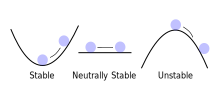
\includegraphics[scale=0.3]
  {Figs/stability_drawing.png}  
  \caption{Intuitive linear stability}
  \label{fig:stability_drawing}
\end{figure}
%----------------------------
\end{frame}
%----------------------------
%----------------------------
\begin{frame}{Linear Stability:}
%----------------------------
 Let $\underline{x}_{0}$ be an equilibrium of $\underline{\dot{x}} = \underline{f}(\underline{x})$.\\
 $\Rightarrow \underline{f}(\underline{x}_{0}) = 0$.\\
 Small perturbation about $\underline{x}_{0} \Rightarrow \underline{x} = \underline{x}_{0} + \underline{\delta x}$\\
 Substituting in the governing equation and using Taylor expansion:\\
 \begin{align*}
  \underline{\dot{x}} &= \underline{f}(\underline{x})\\
  %
  \cancelto{0}{\underline{\dot{x}_{0}}} + \underline{\dot{\delta x}} &= \cancelto{0}{\underline{f}(\underline{x}_{0})} + [DF]|_{\underline{x}_{0}} \underline{\delta x} + h.o.t. (O(\underline{\delta x}^{2}))\\
  %
  \underline{\dot{\delta x}} &= \underbrace{[DF]|_{x_{0}}}_{\text{Stability Matrix } A} \underline{\delta x}
 \end{align*}
 We obtained a ``linearized'' system around $\underline{x}_{0}$
 where the stability matrix $A_{ij} = \frac{\partial f_{i}}{\partial x_{j}}$, evaluated at $\underline{x}_{0}$.
%----------------------------
\end{frame}
%----------------------------
%----------------------------
\begin{frame}{Linear Stability of $1d$ Swift-Hohenberg Equation with quadratic-cubic nonlinearity ($SH23$):}
%----------------------------
$SH23$ is given by:
\begin{equation} \label{eq:sh23}
\frac{\partial u}{\partial t}=
ru-(\partial^{2}_{x}+q_{c}^{2})^{2}u+vu^{2}-gu^{3}
\end{equation}

Here, we choose $q_{c} = 0.5, v = 0.41, g = 1$, in accordance with \cite{burke2007snakes}
Let's find the stationary solutions of Eqn. (\ref{eq:sh23})

\begin{equation}\label{eq:sh23_eqb}
0=   (r-q_{c}^{4})u+vu^{2}-gu^{3}
\end{equation}

%----------------------------
\end{frame}
%----------------------------
%----------------------------
\begin{frame}{Equilibria:}
%----------------------------
\begin{equation}\label{eq:sh23_eqbs}
 u = 0, \quad u_{\pm} = \frac{1}{2g}[v \pm \sqrt{v^{2} + 4g(r-q_{c}^{4})}]
\end{equation}

\begin{figure}[ht]
  \centering
  % include first image
  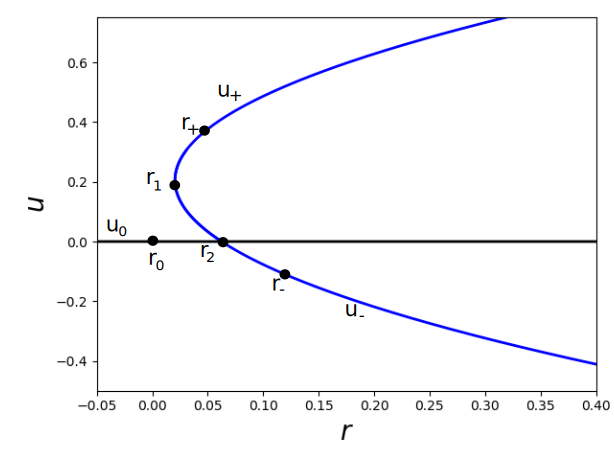
\includegraphics[scale=0.3]
  {Figs/sh.png}  
  \caption{Analytically obtained steady solutions of $SH23$.}
  \label{fig:sh}
\end{figure}
%----------------------------
\end{frame}
%----------------------------
%----------------------------
\begin{frame}{Equilibria:Linear Stability}
%----------------------------
For a stationary solution $u_{s}$, to find stability: substitute 

\begin{equation}\label{eq:linstab_ansatz}
 u = u_{s} + \epsilon\tilde{u}e^{\beta t},
 %
\end{equation}
into Eqn.(\ref{eq:sh23}) and linearize
\begin{equation}\label{eq:eigval_prob}
 \beta \tilde{u} = \mathcal{L}[u_{s}] \tilde{u}, \quad  \tilde{u}(x+L) = \tilde{u}(x),
\end{equation}
%
with $\mathcal{L} = [r - (\partial_{x}^{2} + q_{c}^{2})^{2} + 2 v u_{s}(x) - 3gu_{s}^{2}(x) ]$.
%----------------------------
\end{frame}
%----------------------------
%----------------------------
\begin{frame}{Equilibria:Linear Stability}
%----------------------------
The eigenfunctions of Eqn.(\ref{eq:eigval_prob}) are $\sin{kx}, \cos{kx}$ for $u_{0}, u_{\pm}$ and we can find their corresponding growth rates $\beta_{0}, \beta_{\pm}$. 
\begin{align}
 & \beta_{0} = r - (q_{c}^{2}-k^{2})^{2}\\
 %
 &\beta_{\pm} = 3q_{c}^{4} - (q_{c}^{2}-k^{2})^{2} - 2r - \frac{v}{2g}\left[v \pm \sqrt{v^{2} + 4g(r-q_{c}^{4})}\right].
\end{align}

%----------------------------
\end{frame}
%----------------------------
%----------------------------
\begin{frame}{Equilibria: Linear Stability}
%----------------------------
$u_{\pm}$ branches are generated at $r = r_{1} = q^{4}- v^{2}/4g$ in a saddle-node bifurcation. $u_{-}$ branch bifurcates from the trivial solution $u_{0}$ at $r = r_{2} = q_{c}^{4}$ in a transcritical bifurcation.  

%----------------------------
\end{frame}
%----------------------------
%----------------------------
\begin{frame}{Trivial solution: perturbation theory, Method of multiple scales}
%----------------------------
Define small parameter $r = - \epsilon^{2} \mu_{2}$, ($\mu_{2} > 0$) and look for stationary solutions of Eqn. \ref{eq:sh23} of the form:
\begin{equation}
u_{s}(x)=\epsilon u_{1}(x, X)+\epsilon^{2} u_{2}(x, X)+\hdots
\end{equation}
where $X = \epsilon x$ is the slow space-scale.
%----------------------------
\end{frame}
%----------------------------
%----------------------------
\begin{frame}{Trivial solution: perturbation theory, Method of multiple scales}
%----------------------------
\begin{subequations}\label{eq22}
    \begin{equation}
        \frac{d}{dx}=\frac{\partial}{\partial x_{0}}+\epsilon\frac{\partial}{\partial x_{1}}
    \end{equation}
    
    \begin{equation}
        \frac{d^{2}}{dx^{2}}=\frac{d}{dx}(\frac{d}{dx})=\frac{\partial^{2}}{\partial x_{0}^{2}}+2\epsilon\frac{\partial}{\partial x_{0}\partial {x_{1}}}+\epsilon^{2}\frac{\partial^{2}}{\partial x_{1}^{2}}
    \end{equation}
    
    \begin{equation}
        \frac{d^{3}}{dx^{3}}=\frac{\partial^{3}}{\partial x_{0}^{3}}+3 \epsilon \frac{\partial^{3}}{\partial x_{0}^{2}\partial x_{1}}+3\epsilon^{2}\frac{\partial^{3}}{\partial x_{1}^{2}\partial x_{0}}+\epsilon^{3}\frac{\partial^{3}}{\partial x_{1}^{3}}
    \end{equation}
    
    \begin{equation}
        \frac{d^{4}}{dx^{4}}=\frac{\partial^{4}}{\partial x_{0}^{4}}+4\epsilon\frac{\partial^{4}}{\partial x_{0}^{3}\partial x_{1}}+6\epsilon^{2}\frac{\partial^{4}}{\partial x_{0}^{2}\partial x_{1}^{2}}+4\epsilon^{3}\frac{\partial^{4}}{\partial x_{0}^{1}\partial x_{0}}+\epsilon^{4}\frac{\partial^{4}}{\partial x_{1}^{4}}
    \end{equation}
\end{subequations}


%----------------------------
\end{frame}
%----------------------------
%----------------------------
\begin{frame}{Trivial solution: Weakly nonlinear perturbation theory}
%----------------------------
 $x_{0} = x$, $x_{1}= X$
\begin{subequations}\label{eq23}
    \begin{equation}
        O(\epsilon): (\partial_{x}^{2}+q_{c}^{2})u_{1}=0
    \end{equation}
    
    \begin{equation}
        O(\epsilon^{2}): -(\partial_{x}^{2}+q_{c}^{2})u_{2}=4\frac{\partial^{4}}{\partial x_{0}^{3}\partial x_{1}}u_{1}+4q_{c}^{2}\frac{\partial}{\partial x_{0}\partial {x_{1}}}u_{1}-vu_{1}^{2}
    \end{equation}
\end{subequations}

We can solve the leading order equation: $\Rightarrow$ 

% \begin{subequations}\label{eq24}
    \begin{equation}
        u_{1}(x,X)=Z_{1}(X)\exp{(iq_{c}x)}
        +h.o.t.
    \end{equation}
%     \begin{equation}
%         u_{2}(x_{0},x_{1})= \frac{2\nu}{q_{c}^{4}} |A_{1}|^{2}+\frac{\nu}{9q_{c}^{4}}A_{1}^{2}exp(2iq_{c}x)+A_{2}(x_{1})exp(iq_{c}x)
%     \end{equation}
% \end{subequations}

%----------------------------
\end{frame}
%----------------------------
%----------------------------
\begin{frame}{Trivial solution: Weakly nonlinear perturbation theory}
%----------------------------
Where the slowly varying envelope amplitude $Z(X, \epsilon) = Z_{1}(X) + \epsilon Z_{2}(X)$ satisfies:
\begin{equation}\label{eq:ampl_eqn}
 4q_{c}^{2}{Z_{1}}_{XX} = \mu_{2}Z_{1} - \gamma_{3}Z_{1}|Z_{1}|^{2}
\end{equation}

 at the leading order (comes from Fredholm's alternative, see \cite{burke2007snakes}, \cite{knobloch2015spatial} for details). Here $\gamma_{3} = \frac{38 v^{2}}{9q_{c}^{4}} - 3g$. Substituting values for our parameters $\gamma_{3} \approx 8.35 > 0 \Rightarrow$ subcritical bifurcation at origin!
%----------------------------
\end{frame}
%----------------------------
%----------------------------
\begin{frame}{Trivial solution: Weakly nonlinear perturbation theory}
%----------------------------
The simplest trivial solution of Eqn.(\ref{eq:ampl_eqn}) is 
\begin{equation}\label{eq:ampl_eqn_soln}
 Z(X) =(\mu_{2}/\gamma_{3})^{1/2} e^{i\phi} + O(\epsilon)
\end{equation}
Spatially periodic solutions of period $L_{c}$ near origin. 

\begin{equation}\label{eq:periodic_states}
 u_{P}(x) = 2 \left(\frac{-r}{\gamma_{3}}\right)^{1/2} \cos{(q_{c}x + \phi)} + O(r) 
\end{equation}

where $\phi$ is an arbitrary phase and $-r > 0 \quad \because \mu_{2} > 0$. 

%----------------------------
\end{frame}
%----------------------------
%----------------------------
\begin{frame}{Trivial solution: Weakly nonlinear perturbation theory}
%----------------------------
Localized solutions - elliptic equations, see \cite{burke2007snakes}. 

\begin{equation}\label{eq:localized_amp}
 Z(X) = \left(\frac{2\mu_{2}}{\gamma_{3}}\right)^{1/2}\sech{\left( \frac{X\sqrt{\mu_{2}}}{2q_{c}}\right)}e^{i\phi} + O(\epsilon)
\end{equation}
and the localized solution corresponds to 
\begin{equation}
 u_{l}(x) = 2 \left(\frac{-2r}{\gamma_{3}}\right)^{1/2}\sech{\left( \frac{X\sqrt{\mu_{2}}}{2q_{c}}\right)}\cos{(q_{c}x + \phi)} + O(r) 
\end{equation}
Phases $\phi = 0, \pi$ `selected' for complicated reasons!
%----------------------------
\end{frame}
%----------------------------
%----------------------------
\begin{frame}{Trivial solution: Weakly nonlinear perturbation theory}
%----------------------------
\begin{figure}[ht]
  \centering
  % include first image
  \includegraphics[scale=0.8]
  {Figs/localized_soln_phases.png}  
  \caption{Phase selection of localized solutions, figure reproduced from\cite{burke2007snakes}.}
  \label{fig:localized_soln_phases}
\end{figure}

%----------------------------
\end{frame}
%----------------------------

%----------------------------
\begin{frame}{Equilibria: Numerical Continuation}
%----------------------------
\begin{figure}[ht]
  \centering
  % include first image
  \includegraphics[scale=0.3]
  {Figs/continuation.png}  
  \caption{Parametric Continuation, see \cite{doedel2007lecture}.}
  \label{fig:continuation}
\end{figure}
%----------------------------
\end{frame}
%----------------------------
%----------------------------
\begin{frame}{Equilibria: Numerical Continuation}
%----------------------------
\begin{figure}[ht]
  \centering
  % include second image
  \includegraphics[scale = 0.4]
  {Figs/pseudo_arclength_continuation.png}  
  \caption{Pseudo arc-length continuation, see \cite{doedel2007lecture}. The dots are now wrt the arc-length $s$.}
  \label{fig:pseudo_arclength_continuation}
\end{figure}
%----------------------------
\end{frame}
%----------------------------

%----------------------------
\begin{frame}{Equilibria: Numerical Continuation}
%----------------------------
\begin{figure}[ht]
  \centering
  % include first image
  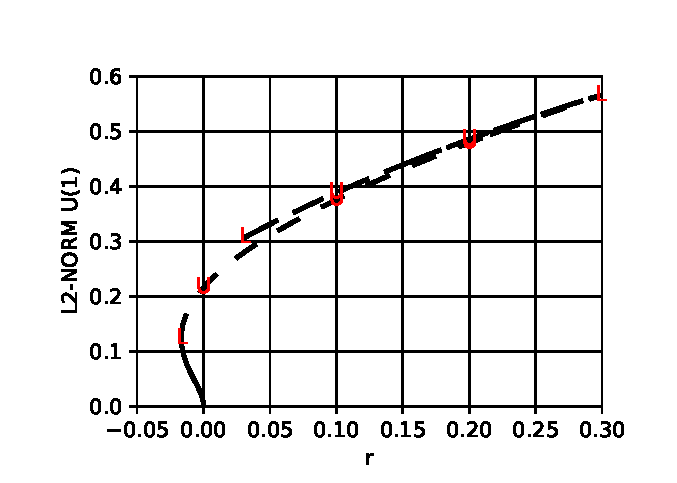
\includegraphics[scale=0.3]
  {Figs/sh11.png}  
  \caption{A new branch emanating from $r_{0}$, obtained via numerical continuation}
  \label{fig:sh11}
\end{figure}
%----------------------------
\end{frame}
%----------------------------
%----------------------------
\begin{frame}{Equilibria: Numerical Continuation}
%----------------------------
\begin{figure}[ht]
\begin{subfigure}{\textwidth}
  \centering
  % include first image
  \includegraphics[scale=0.4]
  {Figs/sh_snaking.png}  
%   \caption{}
\end{subfigure}

\begin{subfigure}{.4\textwidth}
  \centering
  % include first image
  \includegraphics[scale=0.2]
  {Figs/shper_1.png}  
%   \caption{}
  \label{fig:vary_V0}
\end{subfigure}
\begin{subfigure}{.4\textwidth}
  \centering
  % include second image
  \includegraphics[scale = 0.2]
  {Figs/shper_2.png}  
%   \caption{}
  \label{fig:vary_B}
\end{subfigure}
\caption{Snaking, level:noob.}
\label{fig:sh_snaking}
\end{figure}

%----------------------------
\end{frame}
%----------------------------
%----------------------------
\begin{frame}{Equilibria: Numerical Continuation}
%----------------------------
\begin{figure}[ht]
  \centering
  % include first image
  \includegraphics[scale=0.5]
  {Figs/sh_snaking_real.png}  
  \caption{Snakes and ladders, obtained from \cite{knobloch2015spatial}, level:pro.}
  \label{fig:sh_snaking_real}
\end{figure}

%----------------------------
\end{frame}
%----------------------------
%----------------------------
\section{Geometric/Dynamical Systems Explaination:}
%----------------------------
%----------------------------
\begin{frame}{Geometric/Dynamical Systems Explaination:}
%----------------------------

\begin{figure}[ht]
\begin{subfigure}{\textwidth}
  \centering
  % include first image
  \includegraphics[scale=0.4]
  {Figs/nonsnaking_scenario.png}  
  \caption{Non-snaking scenario.}
  \label{fig:nonsnaking_scenario}
\end{subfigure}
\begin{subfigure}{\textwidth}
  \centering
  % include second image
  \includegraphics[scale = 0.4]
  {Figs/snaking_scenario.png}  
  \caption{Snaking scenario.}
  \label{fig:snaking_scenario}
\end{subfigure}
\caption{Non-snaking vs snaking scenario, see \cite{lloyd2008localized}.}
\label{fig:snaking_vs_nonsnaking}
\end{figure}
%----------------------------
\end{frame}
%----------------------------

%----------------------------
\begin{frame}{Take-home messages:}
%----------------------------
\begin{itemize}
 \item Localized patterns are ubiquitous in nature.
 \item Linear stability analysis comes in handy to produce the skeleton of the bifurcation diagram and provides insights.
 \item Weakly nonlinear analysis can tell the nature of bifurcations near equilibria.
 \item The dynamics can be understood as a (spatial) homoclinic orbit of the trivial solution that visits the neighborhood of the periodic pattern (a spatial periodic orbit).
\end{itemize}
%----------------------------
\end{frame}
%----------------------------

%----------------------------
\begin{frame}{References}
%----------------------------
\bibliography{bib/bibliography}
%----------------------------

%----------------------------
\end{frame}
%----------------------------


\end{document}
